\section{Permerability and Darcy's law}
\label{sec:darcy_law}
When applying a pressure difference on each side of some porous material filled with a fluid, the fluid will start to flow in the direction of lower pressure. In 1856, H. Darcy found a linear relation between the pressure difference and the fluid flow rate. This relation is called Darcy's law and tells us what volumetric flow rate (how many cubic meters of fluid per second) $Q$ we can expect from an \textit{incompressible} fluid with dynamic viscosity $\mu$ through a material of length $L$, \textit{permeability} $k$ (discussed further in section \ref{sec:permeability}) and volume $V$ when we apply a pressure difference $\Delta P$, see figure \ref{fig:darcys_law}. 
\begin{figure}[h]
\begin{center}
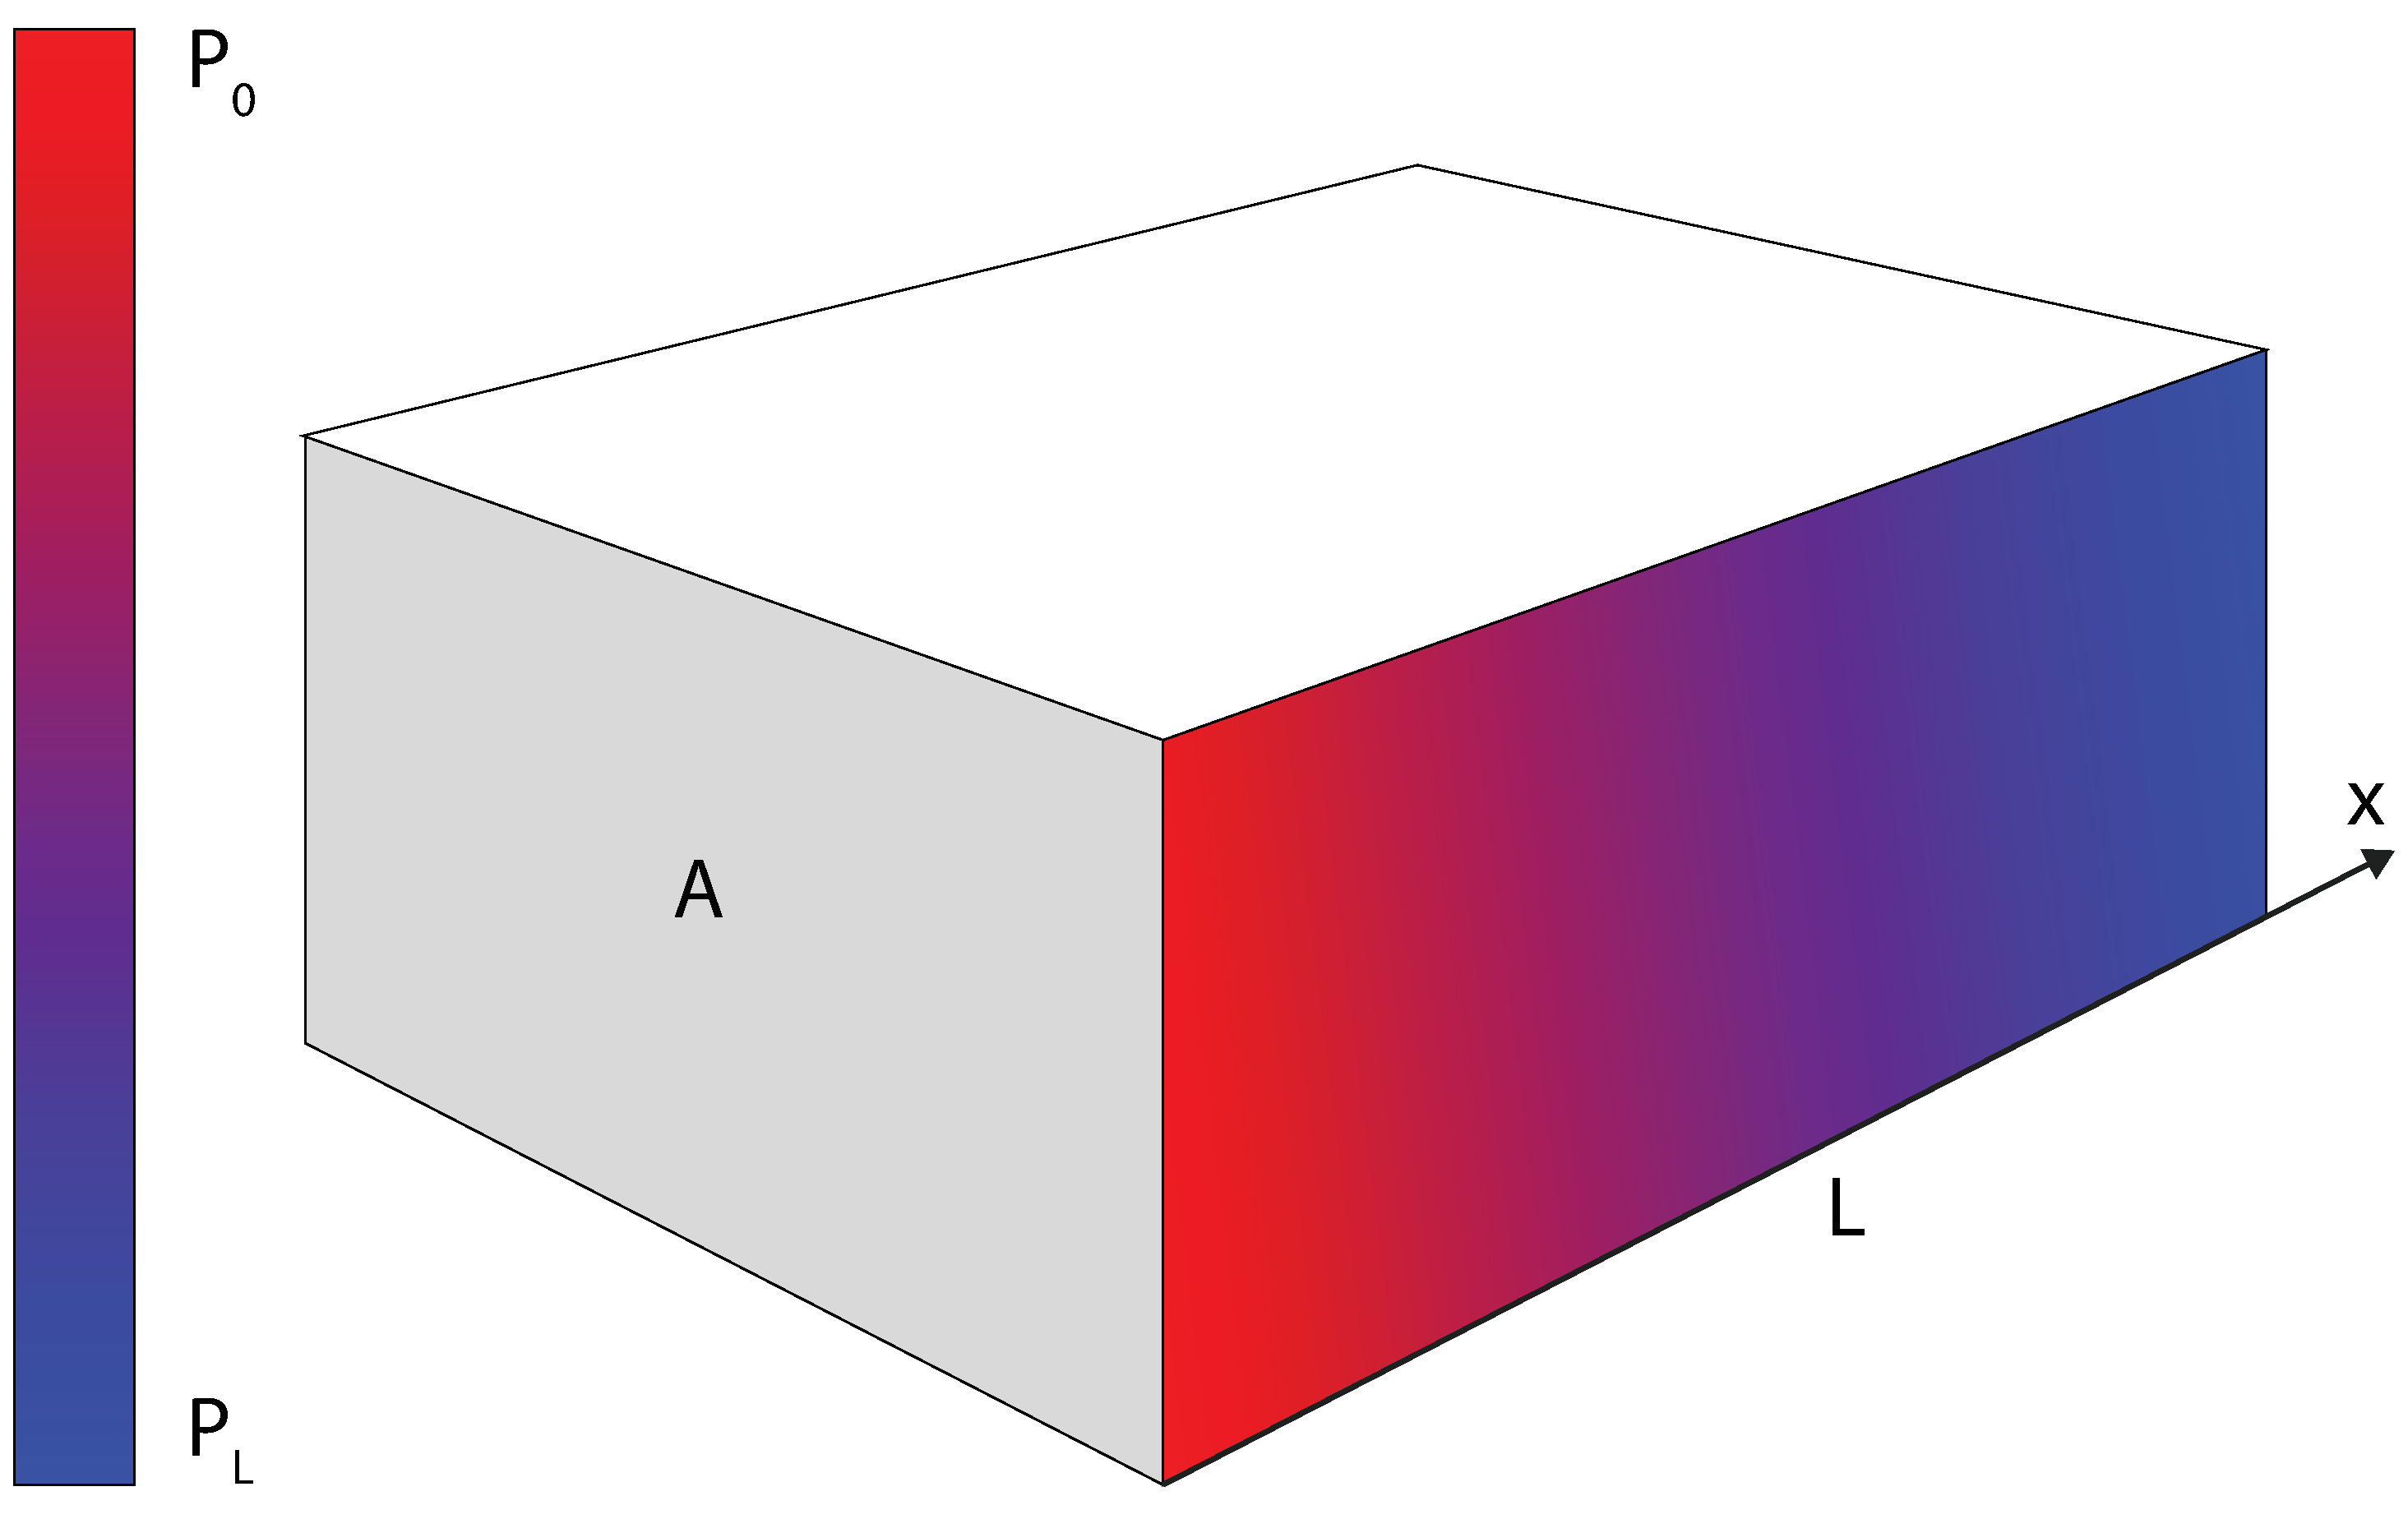
\includegraphics[width=\textwidth, trim=0cm 0cm 0cm 0cm, clip]{kinetic_theory/figures/darcy.eps}
\label{fig:darcys_law}
\end{center}
\caption{A box with volume $V=LA$ with fixed pressure values at $x=0$ and $x=L$. The volumetric flow rate $Q$ through a cross sectional area $A$ is given by Darcy's law in equation \eqref{eq:darcy_2}}.
\end{figure}
The one dimensional version of Darcy's equation is given as 
\begin{align}
\label{eq:darcy_1}
	u = {Q\over A} = {k\over \mu}{\Delta P\over L},
\end{align}
where $u$ is the \textit{volumetric flux} (volumetric flow rate per unit area), $\Delta P = P_0 - P_L \geq 0$ is the pressure difference, $A$ is the cross sectional area; the area of the material orthogonal on the flow direction and $L$ is the length of the material in the flow direction. By letting $L\rightarrow 0$, we get the differential form of Darcy's law
\begin{align}
\label{eq:darcy_2}
	u = -{k\over \mu}{\nabla P},
\end{align}
where we picked up a minus sign because the fluid flows from high pressure to low pressure. 


\section{Permeability $k$}
\label{sec:permeability}
The motivation of introducing the concept permeability is to separate the proportionality constant $\sigma_D = k/\mu$ in equation \eqref{eq:darcy_2} into two parts; one that depends on the liquid only, the viscosity $\mu$, and a material specific constant $k$ which we call permeability. This means that we in principle can do an experiment with a liquid with known viscosity, say water, and measure the permeability of some material (Darcy studied a sand filled cylinder in his original experiment). Once you know the permeability, you are able to predict the flow rate through the material for \textit{any} other liquid with a well known viscosity. This is of great importance for i.e. the oil industry where they ideally would like to take a sample of the rock in which the oil and/or gas is confined in, calculate the permeability of the rock to be able to predict the recovery rate.\\
This is of course not completely true in all circumstances. While Darcy originally found the relation as an empiric equation based on experiments, it can be derived from the Navier-Stokes equations. Darcy's law is only correct if the fluid flow satisfies the no-slip condition. As discussed in section \ref{sec:slip_length}, the velocity of a fluid near the surface is proportional to the mean free path $\lambda$, and is often a non-zero quantity in dilute gases. \todo{Show this relation in the no-slip section.} 

\subsection{Klinkenberg effect}
In 1941, L.J. Klinkenberg published a paper explaining the discrepancies between Darcy's law and experiment by applying the theory of no-slip \cite{klinkenberg1941permeability}. His discoveries were of great importance in the oil industry since
\begin{aquote}{Klinkenberg, 1941}
	It has become common practice in the oil industry to determine the permeability of core material with dry air; the equipment usually employed for this determination is arranged to operate with the outlet of the sample at or near atmospheric pressure.
\end{aquote}
He introduced a linear scaling function $f_c$ that relates what he called the \textit{absolute permeability} $k_\infty$, the permeability that is measured with a liquid or a high density gas, to the \textit{apparent permeability} $k_a$ which is the permeability that is measured in the lab for i.e. dilute gases. The relation is given as
\begin{align}
	k_a = f_c k_\infty = \left(1 + 4\alpha\text{Kn}\right)k_\infty,
\end{align}
where $\alpha\approx 1.15$ is the no-slip factor in equation \eqref{eq:noslip_sliplength}. We can rewrite Klinkenberg's equation to 
\begin{align}
	k_a = \left(1 + {b\over P}\right)k_\infty,
\end{align}
by using that
\begin{align}
	4\alpha\text{Kn} &= {4\alpha\lambda \over L} = {b\over P},
\end{align}
where $b=4\alpha\lambda P / L$ is called Klinkenberg's gas slippage factor. We see that $b$ is a constant depending on the geometry of the material and the pressure. 
\subsection{Knudsen's correction}
\label{sec:knudsen_correction}
\begin{align}
	\label{eq:knudsen_correction}
	f_c = [1 + \alpha(\text{Kn})\text{Kn}]\left[1 + {4\text{Kn}\over 1 - b\text{Kn}}\right]
\end{align}
